\documentclass[notheorems,9pt, handout]{beamer}

% Packages with options
\usepackage[english]{babel}
\usepackage[mathscr]{euscript}
\usepackage[utf8]{inputenc}

% Primary Packages
\usepackage{amsbsy, amsmath, amssymb, amsthm, bm, commath, chngcntr, dsfont, econometrics, gensymb, graphicx, IEEEtrantools, longtable, marginnote, mathrsfs, mathtools, mdframed, natbib, parskip, pgf, setspace, subfigure, tabularx, textcomp, tikz}

% Rest of the setup is in the "setup_beamer" package
\usepackage{setup_beamer}

% Title, Author, Institute
\title{Econ 103: Probability and Statistics}
\author{Manu Navjeevan}
\institute{UCLA}

%%%%%%%%%%%%%%%%%%%%%%%%%%%%%%%%%%%%%%%%%%%%%

\begin{document}
\frame{\titlepage}
\section{Intro}
\begin{frame}{Content Outline} 
	\ucla{Single Random Variable}
	\begin{itemize}
		\item Discrete and Continuous random variables
		\item Mean, variance, and expectations
	\end{itemize}
	\ucla{Multiple Random Variables}
	\begin{itemize}
		\item Conditional probabilities and conditional means
		\item Covariance and independence
	\end{itemize}
	\ucla{The Normal Distribution}
	\begin{itemize}
		\item Properties and computing probabilities
	\end{itemize}
	\ucla{The Law of Large Numbers and the Central Limit Theorem}
	\begin{itemize}
		\item The sample mean as a random variable
	\end{itemize}
\end{frame}

\begin{frame}{Random Variable} 
	\label{frame:random-variables}
	\ucla{Question:} What is a random variable?

	Intuitively, we can think of a random variable as a model of an outcome that is uncertain. 
	\begin{itemize}
		\item \red{Example:} Flipping a coin, traffic in the morning, etc.
	\end{itemize}
	\onslide<2->{While the outcome is random, the random variable does have a  \emph{distribution}. For any subset of the outcome space, the distribution describes the probability that the random variable takes a value in that subset. 
	\begin{itemize}
		\item \red{Example:} We know that our flipped coin has a 50\% probability of taking a value in the set \(\{H\}\), a 50\% probability of taking a value in the set \(\{T\}\), and a 100\% probability of taking a value in the set \(\{H,T\}\).
\end{itemize}}
\end{frame}

\begin{frame}{Random Variables} 
	\label{frame:rv-statistics}
	\ucla{Question:} Why do we care about random variables? What does this have to do with econometrics?	

	Consider the population of California. Suppose we want to know about the education levels of people in the population.
	\begin{itemize}
		\item<1-> The education level of a randomly selected person in the population is not deterministic. Different people have different levels of education. 
		\item<2-> We can think about the education level as a \emph{random variable} with a distribution that describes the probability that a randomly selected person has an education level in certain range.
		\begin{itemize}
			\item i.e 30\% of people have high school diplomas, 40\% of people have college degrees, etc. 
		\end{itemize}
		\item<3-> In general however, we may not know the exact distribution of the random variable. Econometrics is about using a random sample of data to make inferences about the underlying distribution of the random variable.
	\end{itemize}
\end{frame}
\section{Single Random Variables}
\begin{frame}{Single Random Variables: Outcome Spaces} 
	\label{frame:single-rv}
	\onslide<1->{Let's formalize the discussion above. Let \(X\) denote a random variable. All random variables come equipped with an \emph{outcome space} that contains all the values that the random variable can take up.} 
	\begin{itemize}
		\item<2-> If \(X\) represents the flipping a coin, the outcome space is \(\{H,T\}\).
		\item<3-> If \(X\) represents rolling a die, the outcome space is \(\{1,2,3,4,5,6\}\).
		\item<4-> If \(X\) represents the 100m sprint time (in seconds) of an Olympic athlete, the outcome space may be \([9.5,10.5]\).
	\end{itemize}
	\onslide<5->{If the outcome space of \(X\) is \emph{countable} (think finite), then we say that \(X\) is a \red{discrete random variable}. If the outcome space of \(X\) is \emph{uncountable} (think infinite), we say that \(X\) is a \red{continuous random variable}}.
	\begin{itemize}
		\item<5-> Flipping a coin and rolling a die would be discrete random variables
		\item<5-> The 100m sprint time of an Olympic athlete would be a continuous random variable.
	\end{itemize}
\end{frame}
\begin{frame}{Single Random Variables: Outcome Spaces and Probability} 
	\label{frame:single-rv-outcomes}
	\onslide<1->{In general in this class, we will notate the outcome space of a random variable \(X\) as \(\calO_X\). Let \(2^{\calO_X}\) denote all the subsets of \(\calO_X\). 

	We will typically be interested in the probability that \(X\) takes values in some \(A \in 2^{\calO_X}\) (that is \(A\subseteq \calO_X\)). This probability is a number between 0 and 1 and will be notated as \(\P_X(A)\). We will require the probability \(\P_X(\cdot)\) to satisfy certain properties:}
	\begin{itemize}
		\item<2-> \(\P_X(\calO_X) = 1\) and \(\P_X(\emptyset)=0\).
		\item<3-> \(0 \leq \P_X(A) \leq 1\) for any \(A \in 2^{\calO_X}\).
		\item<4-> If \(A_1,A_2,\dots\) are pairwise disjoint, then \(\P_X(\cup_{i} A_i) = \sum_i \P_X(A_i)\).
	\end{itemize}
	\onslide<5->{When we say we are interested in the \emph{distribution} of the random variable \(X\), we really mean we are interested in \(\P_X(\cdot)\) as viewed as a map from \(2^{\calO_X}\) onto \([0,1]\).}
\end{frame}
\begin{frame}{Single Random Variables: Discrete Random Variables} 
	\label{frame:discrete-intro}
	\onslide<1->{If \(X\) is a \red{discrete random variable} the distribution or probability function \(\P_X\) can be described by the \emph{probability mass function} or \emph{pmf}, \(p_X(\cdot):\calO_X \to [0,1]\).
	\begin{itemize}
		\item Recall that a discrete random variable has a countable (think finite) outcome space
	\end{itemize}}
	\vspace{5mm}

	\onslide<2->{For each element \(a\) of the outcome space (\(a\in\calO_X\)), the probability mass function evaluated at \(a\), \(p_X(a)\), describes the probability that \(X\) takes value \(a\). That is \(p_X(a) = \P_X(\{a\})\)}.
	\vspace{5mm}

	\onslide<3->{By the last property of probability measures, the pmf can be used to recover the probability that \(X\) takes values in any subset \(A\) of the outcomes space \(\calO_X\)
	\[
		\P_X(A) = \sum_{a\in A} \P_X(\{a\}) = \sum_{a\in A}p_X(a) 
	.\]} 
\end{frame}
\begin{frame}{Single Random Variables: Discrete Random Variables} 
	\label{frame:discrete-ex}
	\onslide<1->{Let's see an example of this. Let \(X\) denote the outcome of a fair dice roll. We can describe the distribution of \(X\) via the probability mass function
	\[
		p_X(a) = \begin{cases}
			\frac{1}{6}  & \text{if }a \in \{1,2,3,4,5,6\}  \\
			0 &\text{for any other value of \(a\)}
		\end{cases}
	\]}
	\vspace{1mm}

	\onslide<2->{Let's use the pmf to compute \(\P_X(A)\) for \(A = \{2,4,6\}\), that is use the pmf to compute the probability that \(X\) takes on an even value.}
	\begin{align*}
		\onslide<3->{\P_X(\{2,4,6\}) &= \sum_{a\in \{2,4,6\}} \P_X(\{a\})}\\
		\onslide<4->{&= \sum_{a\in \{2,4,6\}} p_X(a)  }\\
		\onslide<5->{&= \frac{1}{6}+\frac{1}{6}+\frac{1}{6} }\\
		\onslide<6->{&= 1/2}
	\end{align*}
	\onslide<7->{\ucla{Of course, this result is a bit obvious. However, if the die was not fair, we would follow the same procedure to compute this probability.}}
\end{frame}
\begin{frame}{Single Random Variables: Continuous Random Variables} 
	\label{frame:cont-intro}
	\onslide<1->{If \(X\) is a \red{continuous random variable} we cannot use a probability mass function to describe its distribution.}
	\begin{itemize}
		\item<2-> Recall that if \(X\) is a continuous random variable then the outcome space \(\calO_X\) is (uncountably) infinite.
		\item<2-> What would happen if \(\P_X(\{a\}) > 0\) for each \(a \in \calO_X\)?
		\begin{itemize}
			\item<3-> Then for any (uncountable) set \(A\)
				\[
					\P_X(A) = \sum_{a\in A}\P_X(\{a\}) = \infty 
				.\] 
			\item<3-> So we must have \(\P_X(\{a\}) = 0\) for all \(a \in \calO_X\).
		\end{itemize}
		\item<4-> Intuitively, what is the probability that an Olympic sprinters runs the 100m dash in exactly 9.8412312\dots seconds?
		\begin{itemize}
			\item<4-> Basically zero.
		\end{itemize}
	\end{itemize}
	\onslide<5->{This rules out being able to use a pmf to describe the distribution of a continuous random variable.}
\end{frame}
\begin{frame}{Single Random Variables: Continuous Random Variables.} 
	\label{frame:cont-intro2}
	\onslide<1->{If \(X\) is a \red{continuous random variable} we cannot use a probability mass function to describe its distribution.}
	\vspace{5mm} 
	
	\onslide<2->{Instead we will use the probability density function (pdf), \(f_X(\cdot)\) to describe the distribution of \(X\). The pdf is related to the probability measure \(\P_X\) via the following equation:
	\[
		\P_X(a \leq X \leq b) = \int_a^b f_X(x)\,dx
	.\]}
	\vspace{5mm}

	\onslide<3->{The identity above as well as the rules for the probability measure \(\P_X\) can be used to calculate \(\P_X(A)\) for any set \(A\subseteq \calO_X\).} 
\end{frame}
\begin{frame}{Single Random Variables: Continuous Random Variables} 
	\label{frame:cont-ex}
	\onslide<1->{\ucla{Example: }Let \(X\) be a continuous random variable with pdf \(f_X\) given
	\[
		f_X(a) = \begin{cases}
			1 & \text{if } 0\leq a\leq 1 \\
			0 & \text{otherwise }
		\end{cases}	
	\]
	This distribution is called the \emph{uniform distribution} on \([0,1]\).}
	\vspace{1mm}

	\onslide<2->{\ucla{Problem: }What is \(\P_X([0,0.5])\)?}
	
	\onslide<3->{\ucla{Answer: }Use the pdf}
	\begin{align*}
		\onslide<4->{\P_X([0,0.5]) &= \int_0^{0.5} f_X(x)\, dx} \\ 
		\onslide<5->{&= \int_0^{0.5} 1\, dx} \\
		\onslide<6->{&= 0.5 - 0 = 0.5}
	\end{align*}
\end{frame}
\begin{frame}{Single Random Variables: Review} 
	\label{frame:single-rv-review}
	\ucla{Let's recap}:

	\red{Random Variables:}
	\begin{itemize}
		\item Describe an event whose outcome is unknown
		\item Instead we have probabilities that the outcome takes values in a certain set. 
	\end{itemize}
	\onslide<2->{\red{Discrete Random Variable:}
	\begin{itemize}
		\item Random Variable whose  outcome space is countable (think finite)
		\item Distribution/Probability measure completely described by pmf.
		\begin{itemize}
			\item \(p_X(a) = \P_X(\{a\})\)
		\end{itemize}
	\end{itemize}
	}
	\onslide<3->{\red{Continuous Random Variables:}
	\begin{itemize}
		\item Random variable whose outcome space is uncountable (think infinite)
		\item Distribution/Probability measure completely described by pdf
		\begin{itemize}
			\item \(\P_X([a,b]) = \int_a^b f_X(x)\,dx\)
		\end{itemize}
	\end{itemize}
	}	
\end{frame}
\begin{frame}{Single Random Variables} 
	\centering\red{\Large Questions?}	
\end{frame}
\begin{frame}{Single Random Variables: Expectation} 
	\label{frame:srv-mean}
	One property of a random variable that we may be interested in is the \red{expectation} of a random variable. 
	\begin{itemize}
		\item The expectation can be thought of as a generalized concept of a mean.
		\item That is it is the ``average'' value the random variable \(X\) will take, weighted by the probability that \(X\) takes each value
	\end{itemize}
	\onslide<2->{The expectation of \(X\) is denoted \(\E[X]\) or \(\mu_X\) and is calculated via the following
	{\large 
		\begin{table}[htpb]
		\renewcommand{\arraystretch}{1.5}
		\centering
		\begin{tabular}{c|cc}
			Type  & Discrete R.V & Continuous R.V \\
			\hline
			Formula & \(\sum_{a\in\calO_X} a\cdot p_X(a)\) & \( \int_{\calO_X} a\cdot  f_X(a)\,da\)
		\end{tabular}
		\end{table}}
	}
	\onslide<3->{
	\begin{itemize}
		\item Note that the difference between discrete and continuous is just summation vs. integral.
	\end{itemize}}
\end{frame}


\begin{frame}{Single Random Variables: Expectation} 
	\label{frame:srv-mean-ex1}
	Suppose we enter a lottery that pays us \(\$ 100\) with probability \(1/2\), \(\$400\) with probability \(1/4\), and \(\$0\) with probability \(1/4\). We can represent the payout of this lottery (in dollars) with a random variable \(X\) whose pmf is given
	\[
		p_X(a) = \begin{cases}
			1/2 & \text{if } a \in \{100\} \\
			1/4 & \text{if } a \in \{0,400\} \\
			0 & \text{otherwise} 
		\end{cases}	
	.\] 
	\onslide<2->{Let's calculate the \emph{expected value} of this lottery, or \(\E[X]\). This is the average amount we can expect to win by playing this lottery.}
	\onslide<3->{Using the formula from the slide above:}
	\begin{align*}
		\onslide<3->{\E[X] &= \sum_{a\in \{0,100,400\}}a\cdot p_X(a)}\\
		\onslide<4->{&= 0\cdot\frac{1}{4} + 100\cdot\frac{1}{2} + 400\cdot\frac{1}{4}}\\
		\onslide<5->{&= 50 + 100 = \red{150}}
	\end{align*}
	\onslide<5->{We can expect to win about \$150 by playing this lottery}
\end{frame}
\begin{frame}{Single Random Variables: Expectation} 
	\label{frame:srv-mean-ex2}
	\onslide<+->
	Let's consider the uniform distribution from before. That is, let \(X\) be continuously distributed with outcome space \(\calO_X=[0,1]\) and pdf given by 
	\[
		f_X(a) = \begin{cases}
			1 & \text{if }0\leq a\leq 1 \\
			0 & \text{otherwise }
		\end{cases}
	\] 
	\onslide<+->
	Suppose we want to calculate \(\E[X]\). Using the formula
	\begin{align*}
		\E[X] &= \int_{\calO_X} a\cdot f_X(a)\,da \\
		\onslide<+->{&= \int_{0}^{1} a\cdot 1\,da \\}
		\onslide<+->{&= \frac{a^2}{2}\bigg|_0^1 \\}
		\onslide<+->{&= \frac{1}{2} - 0 = \red{\frac{1}{2}}}  
	\end{align*}
	\onslide<+->
	So the expected value of \(X\) is \(\frac{1}{2}\). There are many ways to interpret this expected value, the most straightforward for me is the average amount you can expect to win from a lottery whose payouts follow the distribution of \(X\). 
\end{frame}


\begin{frame}{Single Random Variables: Expectation} 
	\label{frame:srv-mean2}
	\onslide<+->
	We can generalize this concept a bit further and consider the mean of any function \(g(X)\), which is typically denoted \(\E[g(X)]\).
	\begin{itemize}
		\item Note that \(g(X)\) itself is a random variable. It's outcome is not deterministic but rather follows a distribution based on \(X\).
		\item As with the normal expectation, we can think about this as the average value of \(g(X)\). 
	\end{itemize}
	\onslide<+->
	The formula for calculating \(\E[g(X)]\) is basically the same as for calculating \(\E[X]\).
	{\large 
		\begin{table}[htpb]
		\renewcommand{\arraystretch}{1.5}
		\centering
		\begin{tabular}{c|cc}
			Type  & Discrete R.V & Continuous R.V \\
			\hline
			Formula & \(\sum_{a\in\calO_X} g(a)\cdot p_X(a)\) & \( \int_{\calO_X} g(a)\cdot  f_X(a)\,da\)
		\end{tabular}
		\end{table}}
	\onslide<+->
	\vspace{2mm}
	\begin{itemize}
		\item All that has changed here is that we are multiplying the pmf/pdf by \(g(a)\) instead of by \(a\).
	\end{itemize}
\end{frame}
\begin{frame}{Single Random Variables: Expectation} 
	\label{frame:srv-mean-properties}
	The formulas from this generalization also gives us a nice property that we will use later. Recall from the last slide we can calculate \(\E[g(X)]\) using:
	{\large 
		\begin{table}[htpb]
		\renewcommand{\arraystretch}{1.5}
		\centering
		\begin{tabular}{c|cc}
			Type  & Discrete R.V & Continuous R.V \\
			\hline
			Formula & \(\sum_{a\in\calO_X} g(a)\cdot p_X(a)\) & \( \int_{\calO_X} g(a)\cdot  f_X(a)\,da\)
		\end{tabular}
		\end{table}}
	\onslide<2->
	\vspace{5mm}

	It is then straightforward to see the following: 
	\begin{align*}
		\E[ag(X)+bh(X)] &= a\E[g(X)] + b\E[h(X)]
	\end{align*}
	for any \(a,b\in\SR\). We will refer to this property as the \red{linearity of the expectation}. Later on when we consider multiple or joint random variables, we will see that this can be naturally extended and for two different random variables \(X\) and \(Y\):
	\[
	    \E[aX+bY] = a\E[X] + b\E[Y]
	.\] 
\end{frame}
\begin{frame}{Single Random Variables: Expectation} 
	\label{frame:srv-mean-ex3}
	\onslide<+->
	Let's return to the uniform distribution from before. Suppose that \(X\) follows the pdf
	\[
		f_X(a) = \begin{cases}
			1 & \text{if }0\leq a\leq 1\\
			0 & \text{otherwise}
		\end{cases}
	\] 
	\onslide<+->
	Suppose we want to calculate \(\E[X^2]\). This is like calculating \(\E[g(X)]\) where \(g(a) = a^2\). Using the formula from before
	\begin{align*}
		\E[X^2] &= \int_{\calO_X} a^2\cdot f_X(a)\,da \\
		\onslide<+->{&=\int_0^1 a^2\cdot 1\,da \\}
		\onslide<+->{&=\frac{a^3}{3}\bigg|_0^1\\}
		\onslide<+->{&=\frac{1}{3}-0 = \red{\frac{1}{3}}}
	\end{align*}
	\onslide<+->
	For an arbitrary random variable \(X\), \(\E[X^2]\) is typically referred to as the \emph{second moment} of \(X\).
\end{frame}
\begin{frame}{Single Random Variables: Variance} 
	\label{frame:srv-variance}
	\onslide<+->
	Now that we can compute \(\E[g(X)]\) for any random variable \(X\) and any function \(g(\cdot)\), we are ready to talk about the variance. 

	The variance of a random variable \(X\) is given by the formula
	\begin{align*}
		\sigma^2_X = \Var(X) &= \E[(X-\E[X])^2] \\
		\intertext{The variance is a measure of the ``spread'' of the random variable \(X\); it represents how far on average \(X\) is from its mean. Using linearity of the expectation the expression above can be simplified:}
		\onslide<+->{
				&= \E[X^2 - 2X\E[X] + (\E[X])^2] \\
				&= \E[X^2]-2\E[X]\E[X] + \E[X]^2\\
				&= \E[X^2] - 2\E[X]^2 + \E[X]^2\\
				&= \E[X^2]-(\E[X])^2}
	\end{align*}
	\onslide<+->
	Typically this last expression is easiest to work with. However, the first expression gives us an important property: the variance is always \(\geq 0\). 

\end{frame}
\begin{frame}{Single Random Variables: Variance} 
	\label{frame:srv-var2}
	\onslide<+->
	From the formula \(\Var(X) = \E[X^2]-(\E[X])^2\) as well as the linearity of the expectation we can see the variance has some nice properties. For any constants \(a,b \in \SR\) and any random variable \(X\) we get that
	\begin{itemize}
		\item \(\Var(X+a) = \Var(X)\)
		\item \(\Var(aX) = a^2\Var(X)\)
	\end{itemize}
	\onslide<+->
	Putting these together gives us: \(\Var(aX+b)= a^2\Var(X)\).
	
	\green{Exercise: See if you can work this out yourselves. It shouldn't take more than a few minutes.}
\end{frame}
\begin{frame}{Single Random Variables: Variance} 
	\label{frame:srv-var3}
	Intuitively, \(\Var(X+a) = \Var(X)\) means that the spread around the mean is not effected by just shifting the mean of the random variable (while otherwise keeping the distribution the same).
	\begin{figure}[htpb]
		\centering
		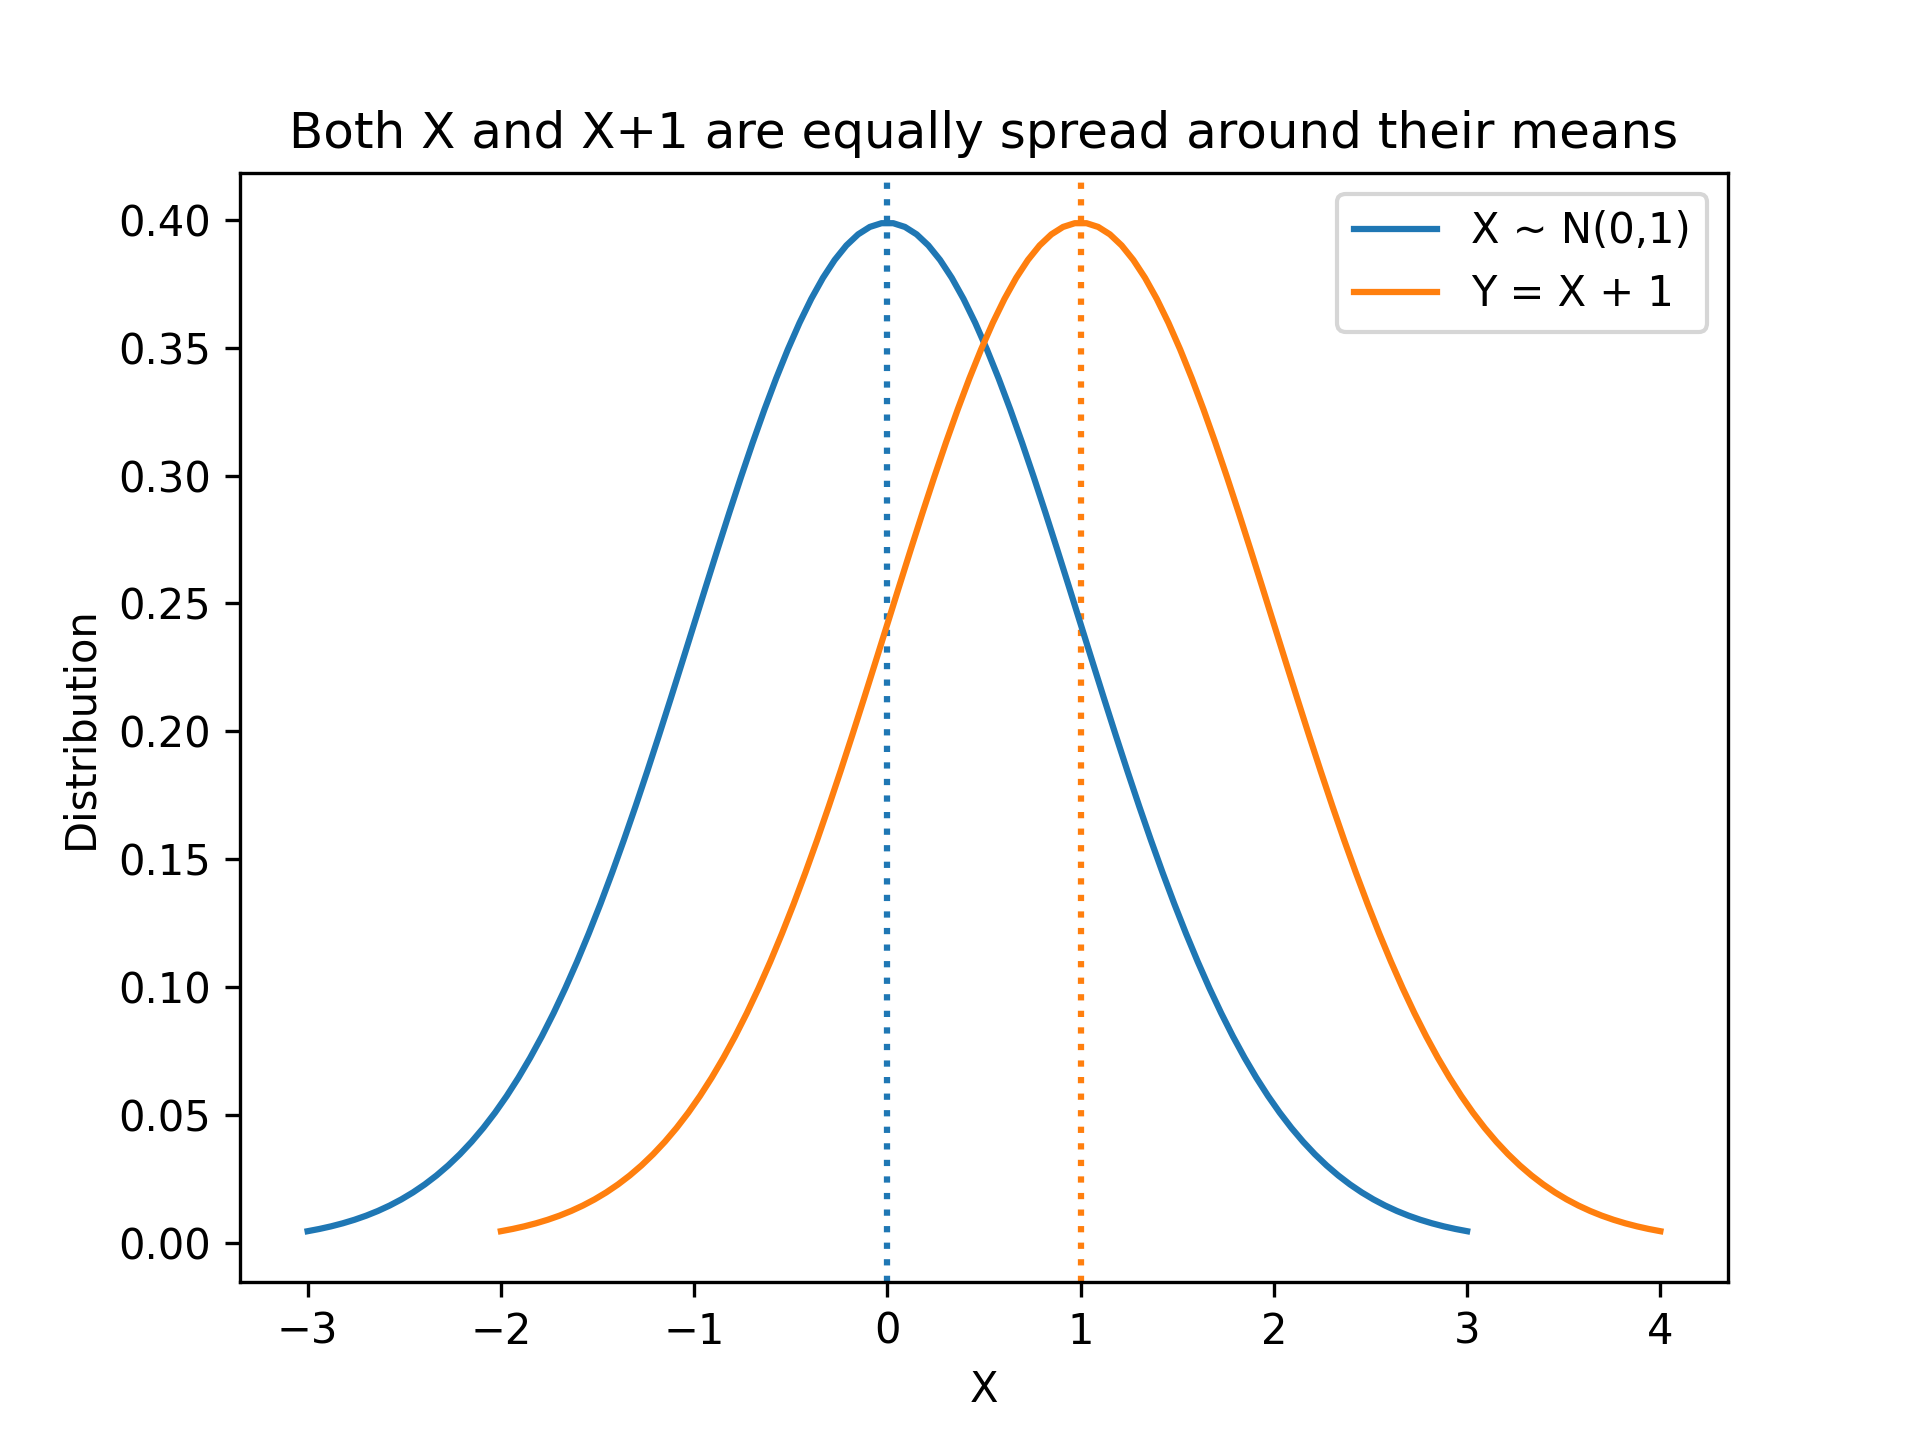
\includegraphics[width=0.7\linewidth]{X-dist.png}
		\caption{Variance remains the same for both variables}%
		\label{fig:X-dist}
	\end{figure}
\end{frame}
\begin{frame}{Single Random Variables: Variance} 
	\label{frame:srv-var4}
	\onslide<+->
	The square root of the variance is denoted 
	\[
	    \sigma_X = \sqrt{\sigma^2_X} = \sqrt{\Var(X)}
	.\] 
	and is called the \red{standard deviation} of \(X\).
\end{frame}
\begin{frame}{Single Random Variables: Variance} 
	\label{frame:srv-var-ex1}
	Let's see this in practice. Suppose we have a lottery that pays \$200 with probability \(\frac{1}{2}\) and nothing (\$0) with probability \(\frac{1}{2} \). The payout of this lottery is a random variable \(X\) with pmf
	\[
	    p_X(a) = \begin{cases}
	    	\frac{1}{2}  & \text{if }a \in \{0,200\}  \\
			0 &\text{otherwise }
	    \end{cases}
	.\] 
	It is straightforward to see that the expected payout of this lottery is \$100, \(\E[X]=100\). 
	\onslide<2->
	However, we may want to know how much we can expect our winnings to deviate from the expected value. That is, we want to know what the variance of the payouts is. 

	Let's compute this two ways, first using the formula \(\Var(X) = \E[(X-\E[X])^2]\) and the second using \(\Var(X)= \E[X^2]-(\E[X])^2\).
\end{frame}
\begin{frame}{Single Random Variables: Variance} 
	\label{frame:srv-var-ex1-2}
	\onslide<1->{
	The payout of this lottery is a random variable \(X\) with pmf
	\[
	    p_X(a) = \begin{cases}
	    	\frac{1}{2}  & \text{if }a \in \{0,200\}  \\
			0 &\text{otherwise }
	    \end{cases}
	.\]}\only<2-6>{First: 
		\begin{align*}
			\Var(X) &= \E[(X-\E[X])^2] \\
			\only<3-6>{ &=\E[(X-100)^2] \\}
			\only<4-6>{&=\sum_{a\in\{0,200\}} (a - 100)^2\cdot p_X(a)\\}
			\only<5-6>{&=(0-100)^2\cdot\frac{1}{2}  + (200-100)^2\cdot\frac{1}{2}\\}
			\only<6>{&= 2\cdot \frac{100^2}{2}=100^2=\red{10000}}
		\end{align*}}\only<7->{Second:
		\begin{align*}
			\Var(X) &= \E[X^2]-(\E[X])^2 \\
			\only<8->{&= \sum_{a\in\{0,200\}}a^2\cdot p_X(a) - 100^2\\}
			\only<9->{&= 0^2\cdot\frac{1}{2} + 200^2\cdot\frac{1}{2} - 100^2 \\}
			\only<10->{&= \frac{(2\cdot 100)^2}{2} - 100^2\\ &= \frac{4}{2}\cdot 100^2 - 100^2 = 100^2 = \red{10000}  }
		\end{align*}
		\only<10->{No matter how we compute it, the variance of this lottery is \(100^2 = 10000\). This makes sense as no matter what happens (win or lose), we are \$100 away from the expected payout.}}
\end{frame}
\begin{frame}{Single Random Variables: Questions?} 
	\label{frame:srv-q2}
	\centering
	\red{\Large Questions?}
\end{frame}
\section{Multiple Random Variables}
\begin{frame}{Multiple Random Variables: Introduction} 
	\label{frame:mrv-intro1}
	Oftentimes we are not only interested in a single random variable, but the relationship between two random variables. In fact this will be the case through the rest of this course:
	\begin{itemize}
		\item We care about the relationship between education and income
		\item We care about the relationship between consumption of a medicine and a health outcome
	\end{itemize}
	\onslide<2->
	In the examples above notice that, not only are the random variables themselves not deterministic 
	\begin{itemize}
		\item not everyone has the same education/income
	\end{itemize}
	but the relationship between the two random variables may not be either
	\begin{itemize}
		\item not everyone who takes a medicine will have the same health outcome
	\end{itemize}
\end{frame}
\begin{frame}{Multiple Random Variables: Introduction} 
	\label{frame:mrv-intro2}
	\ucla{Question:} How do we think about joint random variables?

	\onslide<2->\ucla{Answer:} Much the same as before. Let \((X,Y)\) be a pair of joint random variables. This means there is some outcome space \(\calO_{XY}\) that \((X,Y)\) can take values in and a probability measure \(\P_{XY}(\cdot): 2^{\calO_{XY}}\to[0,1]\) that takes in subsets of the outcome space \(A\subseteq \calO_{XY}\) and gives the probability of both \(X\) and \(Y\) taking values in the set \(A\).
	\begin{itemize}
		\item For example if \(X\) is income and \(Y\) is age, \[\P_{XY}(\{0\leq X\leq 100000, 40\leq Y\leq 42\})\] is the probability that a randomly selected person from the population has an income between \$0 and \$100,000 and is between 40 and 42 years old.
	\end{itemize}
	\onslide<3->
	As before if \(\calO_{XY}\) is countable (finite), we say that \((X,Y)\) are jointly discrete random variables whereas if \(\calO_{XY}\) is uncountable (infinite) we say that \((X,Y)\) are jointly continuous random variables.
\end{frame}

\begin{frame}{Multiple Random Variables: Discrete Random Variables} 
	\label{frame:mrv-intro3}
	Let's quickly go over an example of a joint discrete random variables. As before, the distribution of jointly discrete random variables will be defined by a joint probability mass function. 
	\onslide<2->
	\begin{itemize}
		\item Because we are considering two random variables, \(X,Y\), we can represent the probability mass function as a table
	\end{itemize}
\end{frame}
\begin{frame}{Multiple Random Variables: Discrete Random Variables} 
	\label{frame:mrv-intro4}
	Let \(X\) be a random variable that describes whether a person gets 4 hours of sleep a night, 8 hours a sleep a night, or 12 hours of sleep a night. Let \(Y\) be a random variable that describes whether a person drinks 1 or 2 cups of coffee a day. 

	The joint pmf of \(X\) and \(Y\) can be described with the table below
	\begin{table}[htpb]
		\centering
		\begin{tabular}{c|cc}
			\(p(x,y)\) & 1 cup  & 2 cups\\
			\hline
			4 hours & 0 & 1/6 \\
			8 hours & 1/3 & 1/3 \\
			12 hours & 1/6 & 0
		\end{tabular}
	\end{table}
	Using this table we can see that the probability that a randomly selected person gets 8 hours of sleep and drinks 1 cup of coffee a day is \(1/3\).

	\green{Exercise: What is the probability that a randomly selected person gets 8 hours of sleep?}
\end{frame}

\begin{frame}{Multiple Random Variables: Continuous Random Variables} 
	\label{frame:mrv-cont}
	Now we'll go over an example of a joint continuously distributed random variable. Just like with single random variables, the distribution of a continuous random variable is defined by a probability density function, \(f_{XY}(x,y)\).
	\onslide<2->
	\begin{itemize}
		\item As before, the joint pdf will be related to the joint probability measure \(\P_{XY}(\cdot)\) via the relation
		\[
			\P_{XY}(\{a\leq X\leq b, c\leq Y\leq d\}) = \int_a^b\int_c^d f_{XY}(x,y)\,dy\,dx
		.\] 
	\end{itemize}
\end{frame}
\begin{frame}{Multiple Random Variables: Continuous Random Variables} 
	\label{frame:mrv-cont2}
	Let's consider two sprinters in the 100m dash. Let \(X\) denote the finish time of the \ucla{UCLA} sprinter and \(Y\) denote the finish time of the \red{USC} sprinter. Suppose their times follow the following joint pdf
	\[
		f_{XY}(x,y) = \begin{cases}
			1 & \text{if }9.5\leq x\leq 10.5, 10 \leq y \leq 11 \\
			0 &\text{otherwise}
		\end{cases}
	.\]
	\onslide<2->
	Let's try to find the probability that the UCLA sprinter runs faster than 10 seconds and that the USC sprinter runs faster than 10.5 seconds. That is we want \(\P_{XY}(\{X\leq 10, Y\leq 10.5\})\).
	\onslide<3->
	\begin{align*}
		\P_{XY}(\{X\leq 10,Y\leq 10.5\}) &= \int_{9.5}^{10}\int_{10}^{10.5} f_{XY}(x,y)\,dy\,dx\\
										 &= \int_{9.5}^{10}\int_{10}^{10.5} 1\,dy\,dx\\
										 &= \int_{9.5}^{10}0.5\,dx\\
										 &= 0.5\cdot0.5 = \green{0.25}
	\end{align*}
\end{frame}
\begin{frame}{Multiple Random Variables: Expectations} 
	\label{frame:mrv-expectations}
	Just as before we may want to consider the average or expected value that some function, \(g(X,Y)\), of our joint random variables may take. That is, we want to calculate \(\E[g(X,Y)]\). 
	\onslide<2->

	Here are some examples of functions \(g(x,y)\) for which we may be interested in \(\E[g(X,Y)]\):
	\begin{itemize}
		\item \(g(x,y) = x\implies \E[g(X,Y)] = \E[X]\), the expected value of \(X\)
		\item \(g(x,y) = x-y\implies \E[g(X,Y)]= \E[X-Y]\), the average difference between \(X\) and \(Y\).
		\item \(g(x,y) = \mathds{1}\{x\leq a, y\leq b\}\implies \E[g(X,Y)] = \P_{XY}(\{X\leq a,Y\leq b\})\).
		\item \(g(x,y) = (x-\mu_X)(y-\mu_Y)\implies \E[g(X,Y)]= \Cov(X,Y)\), the covariance between \(X\) and \(Y\).
	\end{itemize}
\end{frame}
\begin{frame}{Multiple Random Variables: Expectations} 
	\label{frame:mrv-expectations2}
	\onslide<+->
	The formula for calculating expected value is the same as before:
	{\large 
		\begin{table}[htpb]
		\renewcommand{\arraystretch}{1.5}
		\centering
		\begin{tabular}{c|cc}
			Type  & Discrete R.V & Continuous R.V \\
			\hline
			Formula & \(\sum_{a,b\in\calO_{XY}} g(a,b)p_{XY}(a,b)\) & \( \int_{X}\int_Y g(a,b)f_{XY}(a,b)\,db\,da\)
		\end{tabular}
		\end{table}}
	\vspace{5mm}
	\ucla{Intuition}: We are evaluating the function at each point in the outcome space and weighting by the probability of that outcome occurring.
	\onslide<+->

	Again note that we have the following linearity of the expectation. For any two functions \(g(x,y)\) and \(h(x,y)\) and any \(a,b\in\SR\):
	\[
		\E[a\cdot g(X,Y) + b\cdot h(X,Y)] = a\E[g(X,Y)] + b\E[h(X,Y)]
	.\] 
	in particular, \(\green{\E[aX+bY] = a\E[X]+b\E[Y]}\).
\end{frame}

\begin{frame}{Multiple Random Variables: Expectations} 
	\label{frame:mrv-expectations-ex1}
	\onslide<+->
	Let's return to the 100m dash example from before, with \(X\) representing the finishing time of the \ucla{UCLA} and \(Y\) representing the finishing time of the \red{USC} sprinter. 
	\[
		f_{XY}(x,y) = \begin{cases}
			1 & \text{if }9.5\leq x\leq 10.5, 10 \leq y \leq 11 \\
			0 &\text{otherwise}
		\end{cases}
	.\]
	Let's try and calculate \(\E[X-Y]\), the expected difference in finishing times between the UCLA and USC sprinters.
	\onslide<+->
	\begin{align*}
		\E[X-Y] &= \int_{9.5}^{10.5} \int_{10}^{11} (x-y)f_{XY}(x,y)\,dy\,dx\\
		\onslide<+->{&= \int_{9.5}^{10.5}\int_{10}^{11} x \,dy\,dx - \int_{9.5}^{10.5}\int_{10}^{11} y\,dy\,dx \\}
		\onslide<+->{&= \int_{9.5}^{10.5} x\,dx - \int_{9.5}^{10.5} \frac{11^2-10^2}{2}\,dx \\}
		\onslide<+->{&= \frac{10.5^2-9.5^2}{2} - 10.5 = \red{-0.5}} 
	\end{align*}
\end{frame}

\begin{frame}{Multiple Random Variables: Covariance} 
	\label{frame:mrv-covariance}
	As mentioned before, a particular expectation we may be interested is the \red{covariance} between \(X\) and \(Y\), defined as 
	\[
		\Cov(X,Y)= \E[(X-\E[X])(Y-\E[Y])]
	.\] 
	The covariance measures how much the variables \(X\) and \(Y\) ``move together'' and will be of particular interest to us in econometrics. It is often notated as \(\sigma_{XY} = \Cov(X,Y)\).
	\onslide<2->

	As before, we can simplify the expression for covariance:
	\begin{align*}
		\Cov(X,Y) &= \E[XY-X\E[Y] - Y\E[X] +\E[X]\E[Y]] \\
				  &= \E[XY] - \E[X]\E[Y] - \E[Y]\E[X] + \E[X]\E[Y] \\
				  &= \E[XY]-\E[X]\E[Y]
  	\end{align*}
\end{frame}
\begin{frame}{Multiple Random Variables: Covariance} 
	\label{frame:mrc-covariance-ex1}
	Let's calculate the covariance between \(X\) and \(Y\) from the example before:
	\[
		f_{XY}(x,y) = \begin{cases}
			1 & \text{if }9.5\leq x\leq 10.5, 10 \leq y \leq 11 \\
			0 &\text{otherwise}
		\end{cases}
	.\]
	From the last exercise we know that \(\E[X] = 10\) and \(\E[Y] = 10.5\). What remains is to calculate \(\E[XY]\):
	\onslide<2->
	\begin{align*}
		\E[XY] &= \int_{9.5}^{10.5}\int_{10}^{11} xy f_{XY}(x,y)\,dy\,dx \\
		\onslide<3->{&= \int_{9.5}^{10.5}x\int_{10}^{11}y\,dy\,dx \\} 
		\onslide<4->{&= \int_{9.5}^{10.5}x\left(\frac{11^2-10^2}{2}\right)\,dx\\}
		\onslide<5->{&= 10.5\left(\frac{10.5^2-9.5^2}{2}\right)= 10.5\cdot 10 = \red{105}}
	\end{align*}
	\onslide<6->
	So \(\Cov(X,Y) = \E[XY] - \E[X]\E[Y] = 105-105=0\). At least to a first order, there is no association between the UCLA sprinters times and the USC sprinters times.
\end{frame}
\begin{frame}{Multiple Random Variables: Covariance} 
	\label{frame:cov-properties}
	From the expression \(\Cov(X,Y) = \E[XY]- \E[X]\E[Y]\), we can see some important properties of the covariance that we will use later on 
	\begin{enumerate}
		\item<1-> \red{Linearity:} \(\Cov(aX,bY) = ab\Cov(X,Y)\)
		\[
			\green{\Cov(aX,bY) = \E[(aX)(bY)] - \E[aX]\E[bY] = ab\left(\E[XY] - \E[X]\E[Y]\right)}
		.\] 
		\item<2-> \red{Symmetry:} \(\Cov(X,Y) = \Cov(Y,X)\) and \(\Cov(X,X) = \Var(X)\)
		\[
			\green{\Cov(X,X) = \E[XX] - \E[X]\E[X] = \E[X^2]-(\E[X])^2 = \Var(X)}
		.\] 
		\item<3-> \red{Sums:} \(\Var(X+Y) = \Var(X) + \Var(Y) + 2\Cov(X,Y)\)
		\begin{align*}
			\green{\Var(X+Y)}\,&\green{=\E[(X+Y)^2] - \E[(X+Y)]^2}	\\
							  &\green{=\E[X^2 + 2XY + Y^2] - \left(\E[X] + \E[Y]\right)^2}\\
							  &\green{=\underbrace{\E[X^2]}_{\Var(X)} + 2\underbrace{\E[XY]}_{\Cov(X,Y)} + \underbrace{\E[Y^2]}_{\Var(Y)} - \underbrace{(\E[X])^2}_{\Var(X)} - 2\underbrace{\E[X]\E[Y]}_{\Cov(X,Y)} - \underbrace{(\E[Y])^2}_{\Var(Y)} }\\
							  &\green{=\Var(X) + \Var(Y) + 2\Cov(X,Y)}
		\end{align*}
	\end{enumerate}
\end{frame}

\begin{frame}{Multiple Random Variables: Covariance} 
	\label{frame:mrc-variance}
	In fact, using the linearity of the covariance, \(\Cov(aX,bY) = ab\Cov(X,Y)\), \(\Var(aX) = a^2\Var(X)\), and \(\Var(bY)  = b^2\Var(Y)\) we can generalize the last property a bit to read
	\begin{align*}
		\ucla{\Var(aX + bY)} &= \Var(aX) + \Var(bY) + 2\Cov(aX,bY) \\ 
							&= \ucla{a^2\Var(X) + b^2\Var(Y) + 2ab\Cov(X,Y)}
	\end{align*}
\end{frame}


\begin{frame}{Multiple Random Variables: Correlation} 
	\label{frame:mrv-correlation}
	Another quantity of interest here is the \red{correlation coefficient} defined as 
	\[
		\rho_{XY} = \frac{\Cov(X,Y)}{\sigma_X\sigma_Y} 
	.\] 
	where we recall that
	\begin{align*}
		\sigma_X &= \sqrt{\sigma_X^2} = \sqrt{\Var(X)} = \sqrt{\E[(X-\E[X])^2]} \\
		\sigma_Y &= \sqrt{\sigma_Y^2} = \sqrt{\Var(Y)} = \sqrt{\E[(Y-\E[Y])^2]}
	\end{align*}
	\onslide<2->
	Calculating the correlation is no more difficult that calculating the covariance, but it is a bit tedious so we won't go over an example right now. 
\end{frame}
\begin{frame}{Multiple Random Variables: Conditioning and Independence} 
	\label{frame:mrv-conditioning}
	Finally, given two joint random variables, \(X\) and \(Y\), we may be interested in characteristics of the distribution of \(Y\) \emph{conditional} on \(X\) taking a certain value. 

	Typically this will be denoted \(\E[Y|X=x]\) and will be called the \red{conditional expectation} of \(Y\) given \(X=x\).
	\onslide<2->
	\begin{itemize}
		\item<2-> We may be interested in the average income for people with college degrees, \(\E[\text{Income} \mid \text{Education = College Graduate}]\)
		\item<3-> We may be interested in the average sales price of a home with floor size 1200 sq. ft, \(\E[\text{Sales Price}\mid\text{Sqft} = 1200]\).
		\item<4-> We may be interested in the average lifespan for smokers, \(\E[\text{Lifespan}\mid\text{Smoker}=1]\).
	\end{itemize}
	\onslide<5->
	In all of these note that knowing the conditional expectation is useful for making predictions as we typically observe the \(X\) variable before we observe the \(Y\) variable.
\end{frame}
\begin{frame}{Multiple Random Variables: Conditioning and Independence} 
	\label{frame:mrv-conditioning-formula}
	Calculating the conditional expectation	essentially involves fixing the \(X\) variable at the point \(X=x\), integrating, and then dividing by the probability that \(X=x\).
	{\large 
		\begin{table}[htpb]
		\renewcommand{\arraystretch}{1.5}
		\centering
		\begin{tabular}{c|cc}
			Type  & Discrete R.V & Continuous R.V \\
			\hline
			\(\E[Y|X=x]\) & \( \frac{\sum_y y\cdot p_{XY}(y,x)}{\sum_y p_{XY}(x,y)}\) & \( \frac{\int_Y y\cdot f_{XY}(x,y)\,dy}{\int_Y f_{XY}(x,y)\,dy}\)
		\end{tabular}
		\end{table}}
	\onslide<2->
	\begin{remark}[]
		Note that \(\sum_y p_{XY}(x,y) = \P_{XY}(\{X=x\})\). We call the quantity \(\int_Y f_{XY}(x,y)\,dy\) the \green{marginal distribution} of \(X\) at \(x\) and denote it \(f_X(x)\).
	\end{remark}
	\onslide<3->
	We see that \(X=x\) is fixed in the above equations while we allow \(Y\) to vary. We then divide by the probability that \(X=x\) (or the density of \(X\) at \(x\), which is the continuous analogue).
	
\end{frame}
\begin{frame}{Multiple Random Variables: Conditioning and Independence} 
	\label{frame:mrv-conditioning-example}
	Let's return to a previous example where \(Y\) is the number of hours of sleep one gets a night and \(X\) is the number of cups of coffee that one drinks a day. 
	
	The joint pmf of \(X\) and \(Y\) can be described with the table below
	\begin{table}[htpb]
		\centering
		\begin{tabular}{c|cc}
			\(p(x,y)\) & 1 cup  & 2 cups\\
			\hline
			4 hours & 0 & 1/6 \\
			8 hours & 1/3 & 1/3 \\
			12 hours & 1/6 & 0
		\end{tabular}
	\end{table}
	\onslide<2->
	Let's compute the number of hours of sleep we can expect someone gets \red{conditional on} them drinking 2 cups of coffee. To this, let's first calculate the probability that one drinks 2 cups of coffee.
	\onslide<3->
	\begin{align*}
		\P_{XY}(\{X=x\}) &=p_{XY}(x,y) = \frac{1}{6} + \frac{1}{3} = \frac{1}{2} 
	\end{align*}
	\onslide<4->
	Now let's fix \(X=2\) and calculate \(\sum_y y\cdot p_{XY}(2,y)\)
	\[
		\sum_y y\cdot p_{XY}(2,y) = 4\cdot \frac{1}{6} + 8\cdot\frac{1}{3} + 12\cdot 0 = \frac{10}{3}   
	.\] 
	\onslide<5->
	Putting this together we find that
	\[
		\E[Y|X=2] = \frac{10}{3}\cdot\frac{2}{1} = \frac{20}{3} \approx 6.6667
	.\] 
\end{frame}
\begin{frame}{Multiple Random Variables: Conditioning and Independence} 
	\label{frame:mrv-independence}
	This is great, but sometimes knowing \(X\) may not help us predict \(Y\). Intuitively, knowledge of \(X\) does not give us any additional knowledge of \(Y\). 

	If this is the case we say that \(X\) is \red{independent} of \(Y\) and denote \(X\perp Y\).

	Some examples of independent random variables:
	\begin{itemize}
		\item<2-> Knowing that one coin flip came up heads doesn't give you any information about the next coin flip, we can say that successive coin flips are independent
		\item<3-> If I buy lottery tickets, whether or not I win the lottery is independent of the color of the shirt I was wearing that day
		\begin{itemize}
			\item<4-> Unless I was wearing my lucky t-shirt
		\end{itemize}
	\end{itemize}
\end{frame}
\begin{frame}{Multiple Random Variables: Conditioning and Independence} 
	\label{frame:mrv-indep-charac}
	There are many characterizations of independence, but for now all we care about are the following implications. If \(X\perp Y\) then:
	\begin{align*}
		\P_{XY}(a\leq X\leq b, c\leq Y\leq d) &= \P_{XY}(a\leq X\leq b)\P_{XY}(c\leq Y\leq d)\;\;\;\forall a,b,c,d\\
		\intertext{and}
		\E[g(Y)|X=x] &= \E[g(Y)]\;\;\;\forall x\in\calO_X, g(\cdot):\calO_Y\to\SR
	\end{align*}
\end{frame}
\begin{frame}{Multiple Random Variables: Conditioning and Independence} 
	\label{frame:mrc-indep-careful}
	Assuming two random variables are independent is useful as the above implications will greatly simplify calculations later on. However, we need to be careful when doing so, as it is a rather strong assumption to make.

	Let's see some examples of variables that seem independent but may not be
	\begin{itemize}
		\item We may think that weather in a city is independent of average rent, is this the case?
		\item Is attending a Greta Thunberg rally independent of your likelihood to attend another climate rally?
	\end{itemize}
\end{frame}
\begin{frame}{Multiple Random Variables: Review} 
	\label{frame:mrv-review}
	\ucla{Let's Recap:}

	\onslide<1->
	\red{Multiple Random Variables:}
	\begin{itemize}
		\item Describe multiple events whose outcomes are unknown.
		\item Have probabilities that the outcomes \green{jointly} take values in arbitrary subsets of the \green{joint} outcome space.
	\end{itemize}

	\onslide<2->
	\red{Expectations:}
	\begin{itemize}
		\item As before describe the ``average'' value of a function of the joint random variables.
		\item The \green{covariance} function is a particular expectation we are interested in as it describes how two variables ``move with'' each other.
	\end{itemize}
	
	\onslide<3->
	\red{Conditioning and Independence:}
	\begin{itemize}
		\item The conditional expectation is the average value of \(Y\) for individuals who have \(X=x\).
		\item If knowing \(X\) does not give us any information on the distribution of \(Y\) we say that \(X\) and \(Y\) are \green{independent}.
	\end{itemize}
\end{frame}
\begin{frame}{Multiple Random Variables} 
	\centering\red{\Large Questions?}	
\end{frame}
\section{The Normal Distribution}
\begin{frame}{The Normal Distribution} 
	\label{frame:nd-into}
	A particular distribution that will be of interest to us is the \red{normal distribution}.
	\begin{definition}[Normal Distribution]
		\label{def:nd}
		A random variable \(X\) follows a normal distribution with mean \(\mu\) and variance \(\sigma^2\) if it is continuously distributed with probability density function (pdf) given by 
		\begin{equation}
			f_X(x) = \frac{1}{\sqrt{2\pi\sigma^2}}\exp\left(-\frac{(x-\mu)^2}{2\sigma^2}\right)
		.\end{equation} 
		If this is the case we denote \(X\sim N(\mu,\sigma^2)\). If \(Z\sim N(0,1)\) we say that \(Z\) follows a \red{standard normal distribution}.	
	\end{definition}
	\begin{figure}[htpb]
		\centering
		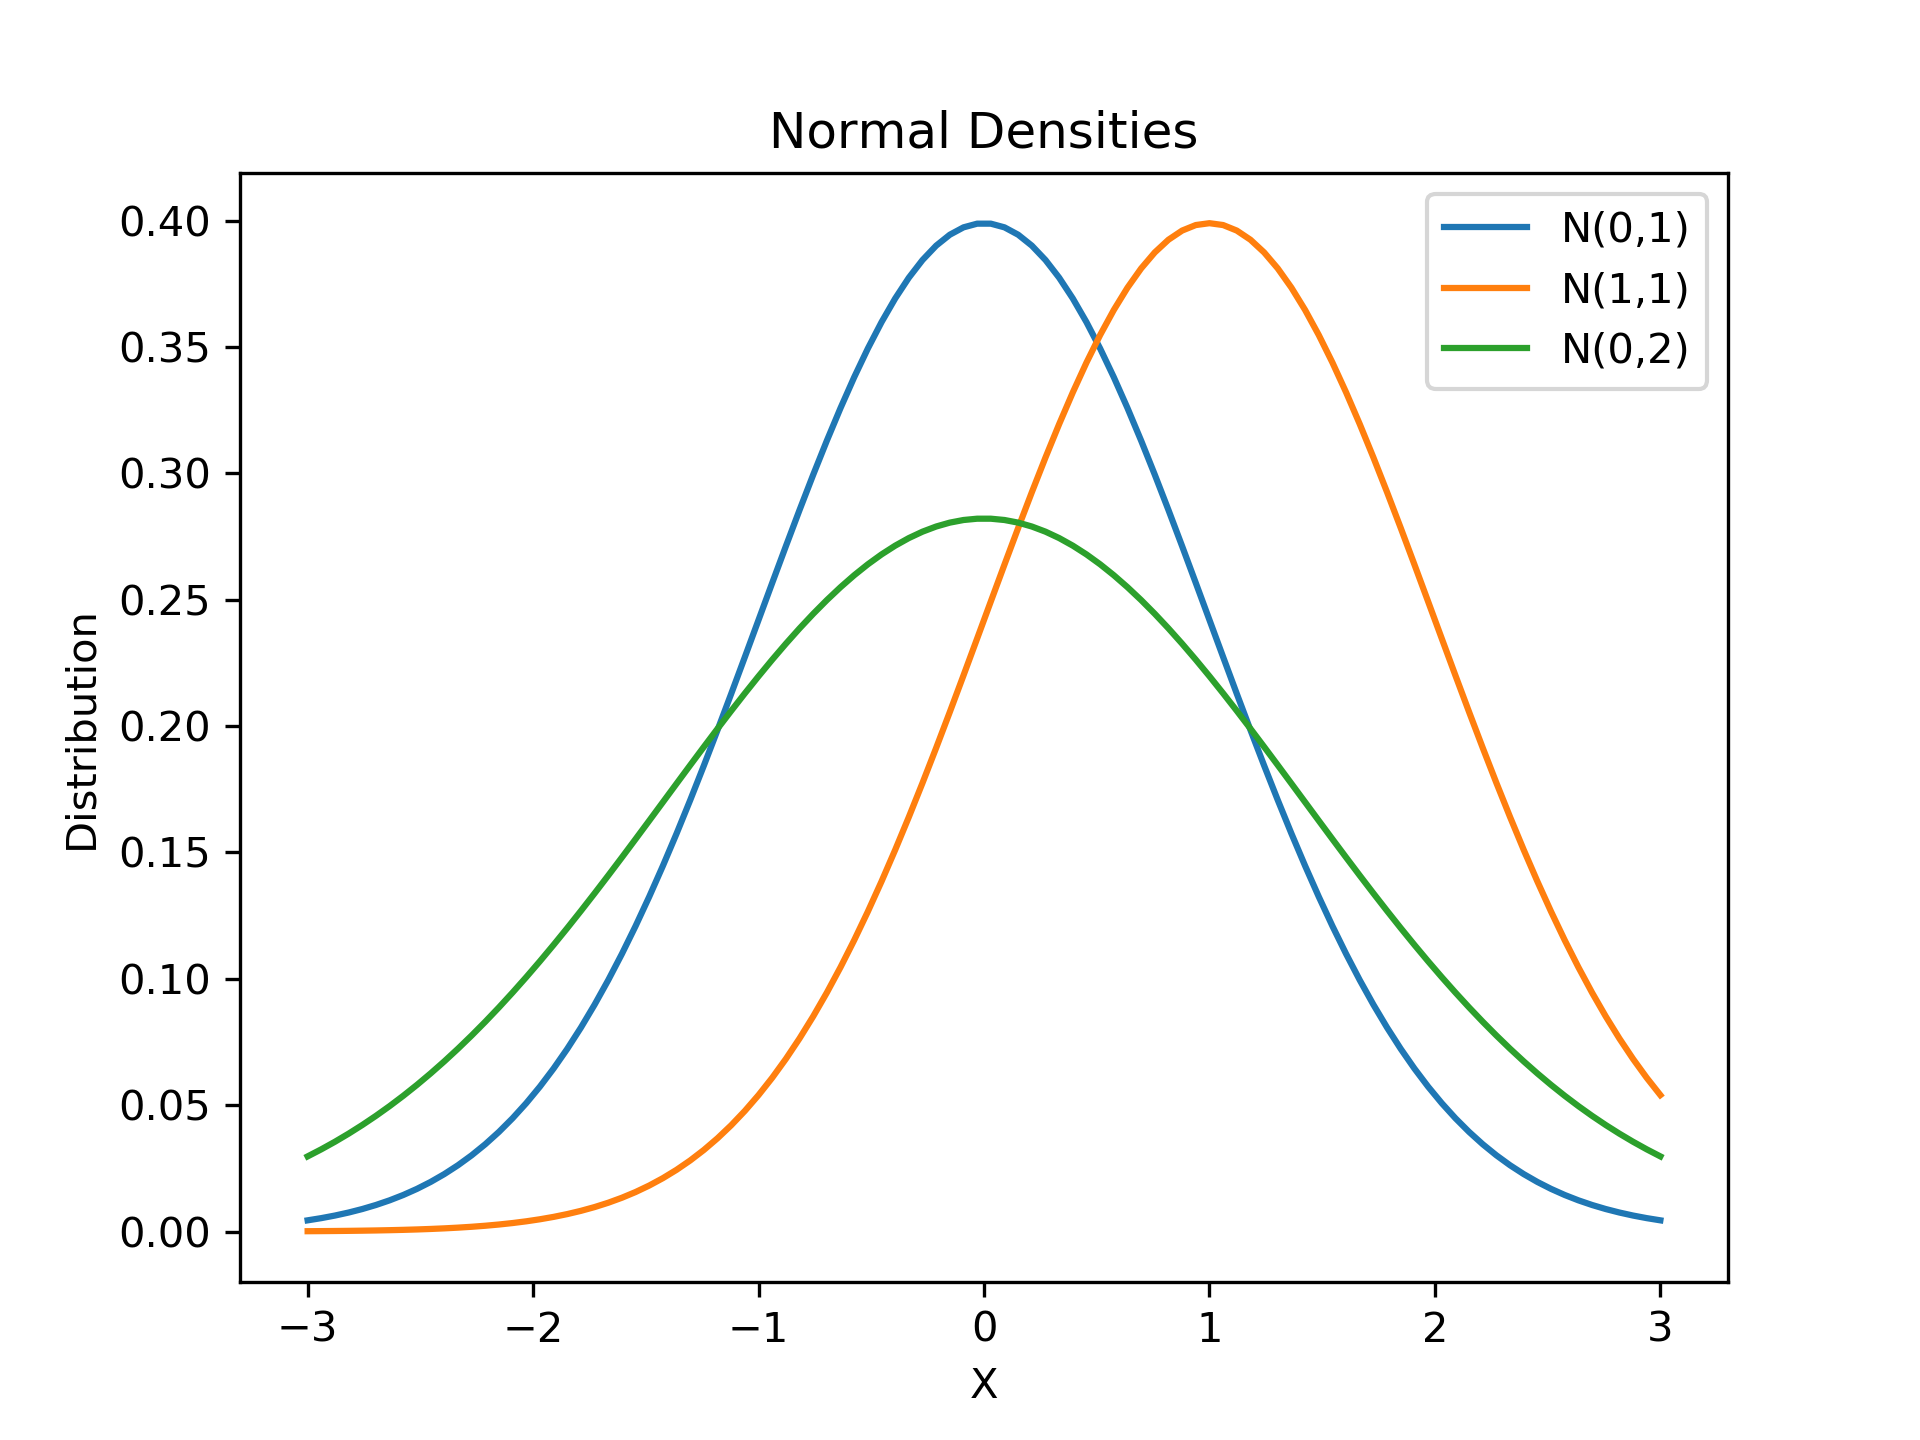
\includegraphics[width=0.4\linewidth]{normal-density.png}	
	\end{figure}
\end{frame}
\begin{frame}{The Normal Distribution: Properties} 
	\label{frame:nd-properties}
	The normal distribution has some useful properties that will be useful later on in the course. We will review them here.
	
	\onslide<2->
	\red{Property 1:} If \(X\sim N(\mu,\sigma^2)\) then \((X-\mu)/\sigma\sim N(0,1)\).

	Why is this property useful? Because it means we can express probabilities for any normal random variable in terms of \(Z\sim N(0,1)\).

	\onslide<3->
	\green{Exercise:} Show that if \(X\sim N(2,100)\) then \(\P(X\geq 22) = \P(Z\geq 2)\).

	\[
		\P(X\geq 22) = \P\left(\frac{X-2}{10} \geq \frac{22 -2}{10} \right) = \P\left(Z \geq 2\right) 
	.\] 
	Here we use the fact that \(\mu=2\) and \(\sigma = \sqrt{100} = 10\).
\end{frame}
\begin{frame}{The Normal Distribution: Properties} 
	\label{frame:nd-properties2}
	\ucla{Question:} This property is great, but how do we calculate \(\P(Z\geq 2)\)?	

	\ucla{Answer:} Either use Z-table or calculate in R. Will cover in lab. 
\end{frame}
\begin{frame}{The Normal Distribution: Properties} 
	\label{frame:nd-properties3}
	\red{Property 2:} If \(X\sim N(\mu_X,\sigma_X^2)\) and \(Y\sim N(\mu_Y,\sigma_Y^2)\) are jointly normal, then \(W=aX+bY\) is also normally distributed for any \(a,b\in\SR\).

	\onslide<2->
	\ucla{What is \(\E[W]\)?}
	\begin{itemize}
		\item Recall by linearity of expectation we have that \(\E[aX+bY] = a\E[X]+ b\E[Y]\)
		\item So, \(\mu_W = \E[W] = a\mu_X + b\mu_Y\).
	\end{itemize}
	\onslide<3->
	\ucla{What is \(\Var(W)\)?}
	\begin{itemize}
		\item Recall that \(\Var(aX+bY) = a^2\Var(X) + b^2\Var(Y) + 2ab\Cov(X,Y)\)
		\item So, \(\Var(W) = \Var(aX+bY) = a^2\sigma_X^2 + b^2\sigma_Y^2 + 2ab\sigma_{XY}\)
	\end{itemize}
	\onslide<4->
	Putting these together we get that
	\[
		W\sim N\left(a\mu_X + b\mu_Y, a^2\sigma_X^2 + b^2\sigma_Y^2 + 2ab\sigma_{XY}\right)
	.\] 
\end{frame}
\begin{frame}{The Normal Distribution: Properties} 
	\label{frame:symmetry}
	\red{Property 3:} The distribution of \(X \sim N(0,\sigma^2)\) is symmetric. That is, for any \(x\), \(\Pr(X \geq x) = \Pr(X \leq -x)\).
	\begin{figure}[htpb]
		\centering
		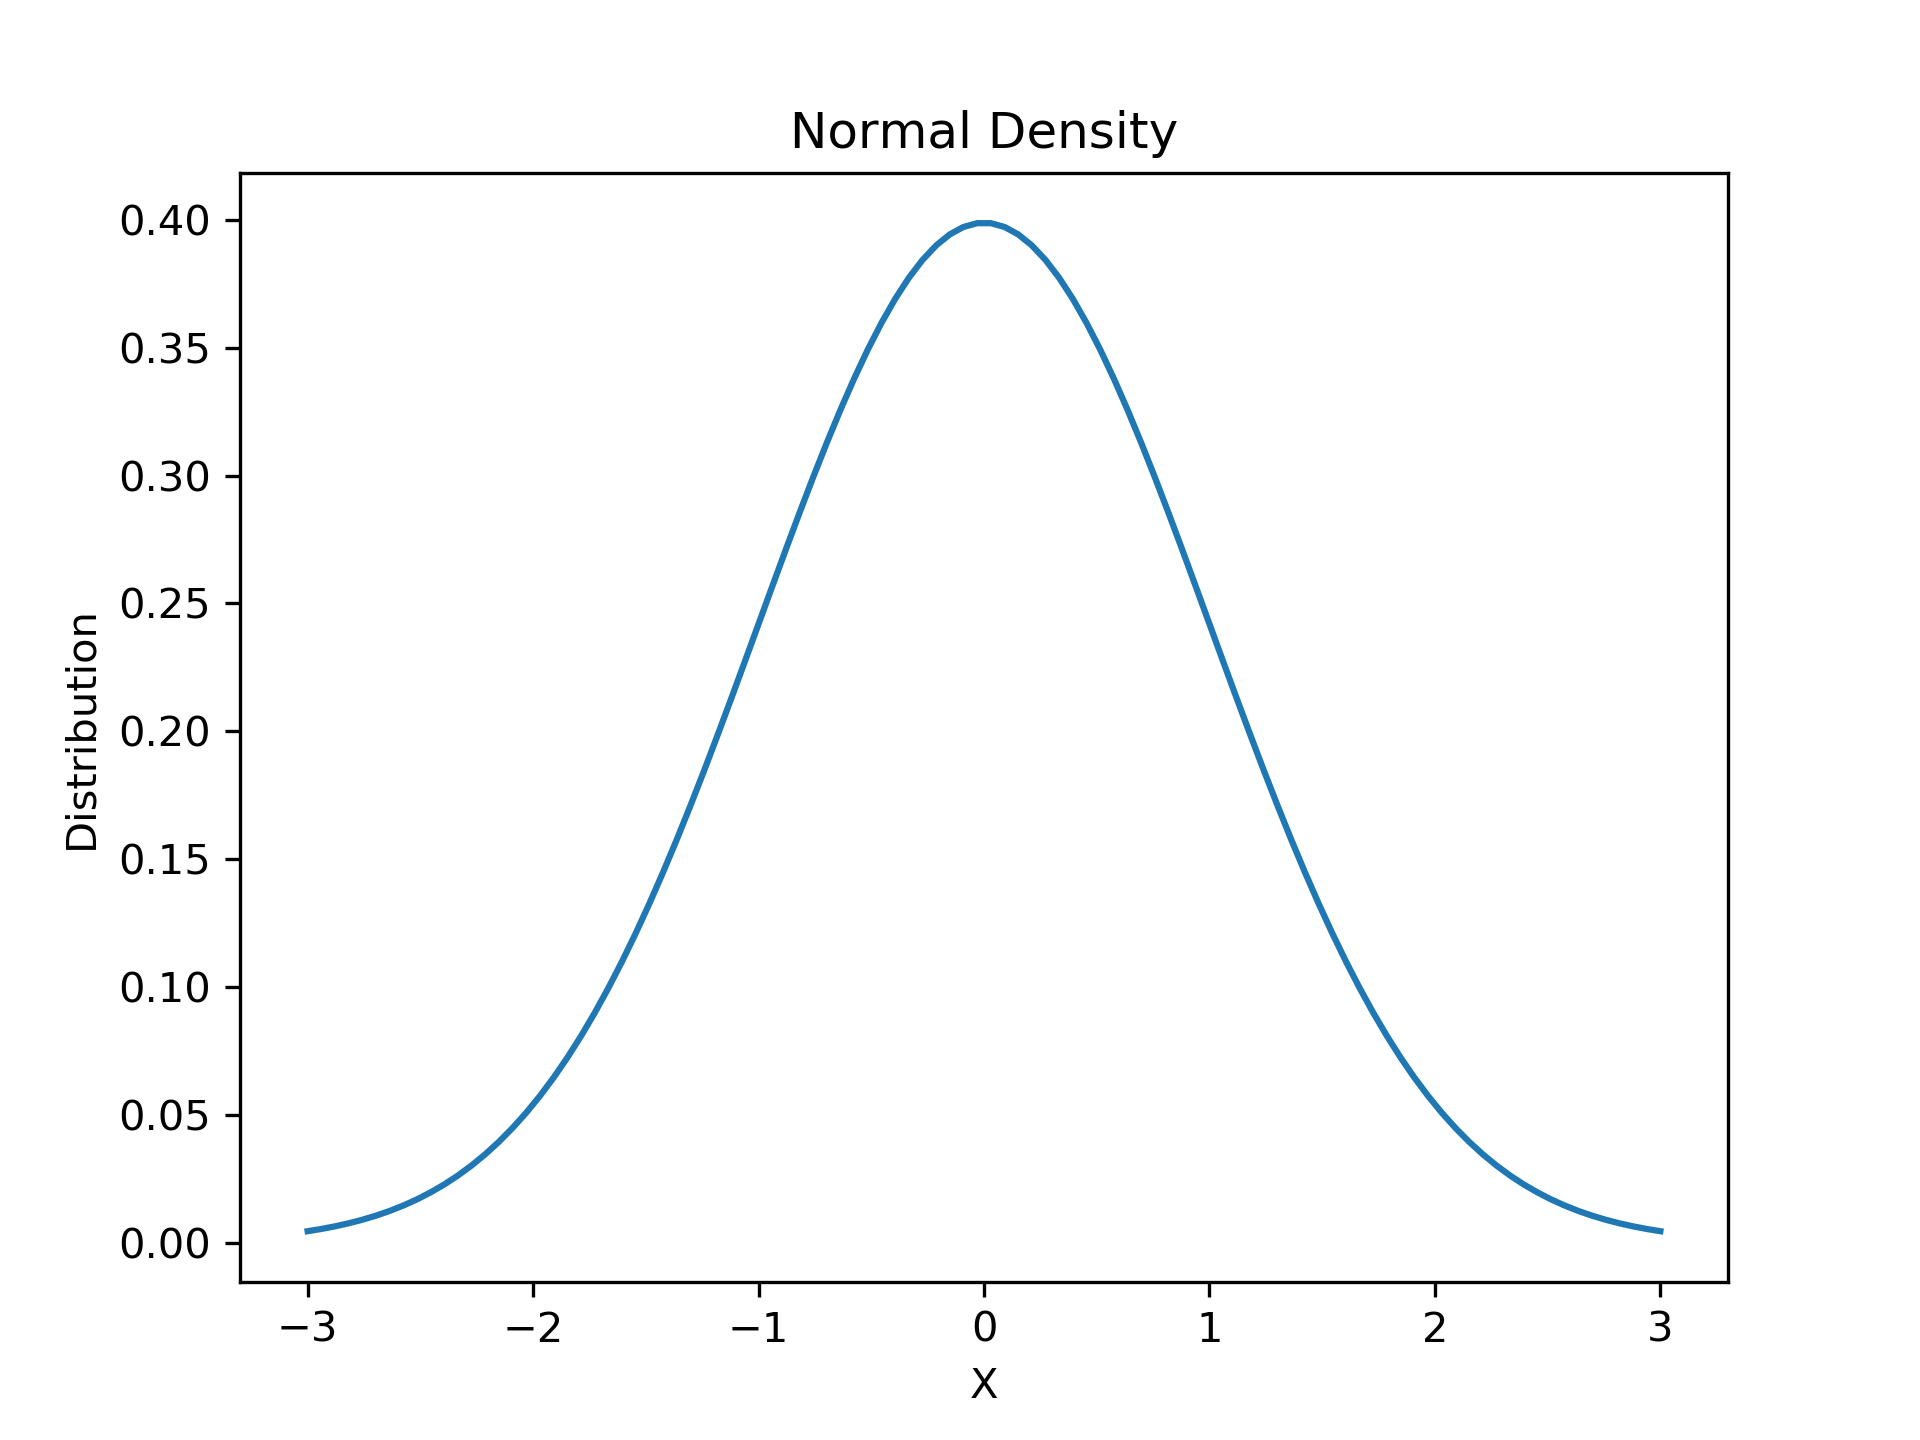
\includegraphics[width=0.50\linewidth]{normal-density-standard.png}
		\caption{Density is symmetric around zero}%
	\end{figure}
	\onslide<2->
	This is useful as it means that if \(X \sim N(0,\sigma_X^2)\) we can compute
	 \[
		 \Pr(|X|\geq c) = \Pr(X\geq c) + \Pr(X \leq -c) = 2\Pr(X\geq c)
	.\] 
\end{frame}

\begin{frame}{The Normal Distribution: Questions} 
	\label{frame:nd-questions}
	\centering
	{\Large
		\red{Questions?}
	}
\end{frame}
\section{The Sample Mean}
\begin{frame}{The Sample Mean} 
	\label{frame:sm-intro}
	\red{Example:} Suppose we are interested in the upcoming ASB election in which Martinez is running against Smith. We randomly selection \(n=100\) students from the population and ask them who they plan on voting for. Answers are recorded as 
	\[
	    X_i = \begin{cases}
	    	1 & \text{if they answer Martinez} \\
			0 & \text{if they answer Smith}
	    \end{cases}
	.\] 
	Based on our sample \(\{X_i\}_{i=1}^{n=100}\) we compute the sample mean (\(\bar X_n\)) and sample variance \(s_n^2\) and find 
	\[
	    \bar X_n = \frac{1}{n}\sum_{i=1}^n X_i = 0.55 \andbox s_n^2 = \frac{1}{n}\sum_{i=1}^n \left(X_i-\bar X_n\right)^2 = 0.25
	.\] 
	\onslide<2->
	\ucla{Questions:}
	\begin{itemize}
		\item<2-> Should we conclude that Martinez will win the election?
		\item<3-> Would we find the same values for \(\bar X_n\) and \(s_n^2\) if we ran the poll again?
		\item<4-> How should we acknowledge the uncertainty in \(\bar X_n\)?
	\end{itemize}
\end{frame}
\begin{frame}{The Sample Mean: As a Random Variable} 
	\begin{center}
		\ucla{Key: Need to think of \(\bar X_n\) and \(s_n^2\) as random variables} 
	\end{center}
	\red{Random Sampling:}
	\begin{itemize}
		\item We think of the sample \(\{X_i\}_{i=1}^n\) as \(n\) different random variables.
		\item Each \(X_i\) is sampled from (has the same distribution as) the population distribution so that \(\E[X_i]=\mu_X\) and \(\Var(X_i)=\sigma_X^2\).
	\end{itemize}
	\onslide<2->
	In the context of the polling example this means that we are interested in the population of voters in the UCLA ASB election. We randomly select \(n=100\) people from this population.
	\begin{itemize}
		\item The identities of each of these people sampled is random.
		\item We would like to use this random sample to learn about the population.
	\end{itemize}
\end{frame}
\begin{frame}{The Sample Mean: As a Random Variable} 
	Random sampling let's us learn about the population by looking at our sample. 
	{\large 
		\begin{table}[htpb]
		\renewcommand{\arraystretch}{1.5}
		\centering
		\begin{tabular}{c|cc}
			& Sample & Population \\
			\hline
			Measure of center & \(\bar X_n\) & \(\E[X]\)\\
			Measure of spread & \(s_n^2\) & \(\Var(X)\)
		\end{tabular}
		\end{table}}
	But, to make the connection precise we must understand the distribution of \(\bar X_n\). Let's start by getting the mean and variance of \(\bar X_n\).
	\onslide<2->
	\begin{enumerate}
		\item<2-> \ucla{The expectation of \(\bar X_n\) is given \(\E[\bar X_n] = \E[X]\).}
		\[
			\green{\E[\bar X_n] = \E[\frac{1}{n}\sum_{i=1}^n X_i] = \frac{1}{n}\sum_{i=1}^n \E[X_i] = \E[X]}
		.\] 
	\item<3-> \ucla{The variance of \(\bar X_n\) is given \(\Var(\bar X_n) = \sigma_X^2/n\).}
		\[
			\green{\Var(\bar X_n) = \Var(\frac{1}{n}\sum_{i=1}^n X_i) = \frac{1}{n^2}\Var(\sum_{i=1}^n X_i^2) = \frac{1}{n^2}\sum_{i=1}^n \Var(X) = \sigma_X^2/n}
		.\] 
		Note that \(\Var(\bar X_n)\to 0\) as \(n\to\infty\). This is the basis of the \red{Law of Large Numbers} which states that \(\bar X_n \to \mu_X\) as \(n\to\infty\).
	\end{enumerate}
\end{frame}
\begin{frame}{The Sample Mean: Central Limit Theorem} 
	\label{frame:clt1}
	\ucla{Question: We know the mean and variance of \(\bar X_n\) but what is it's distribution?}
	\begin{itemize}
		\item Knowing the distribution of the sample mean is useful for computing say 
		\[
			\P\left(|\bar X_n - \E[X]| > 0.05\right)
		\] 
		which is in turn a useful quantity to know for using \(\bar X_n\) to make inferences about \(\E[X]\).
	\end{itemize}
	\onslide<2->
	\ucla{Answer: Central limit theorem tells us that for \(n\) sufficiently large \[\bar X_n \sim N(\mu_x, \sigma_X^2/n)\]}
	\begin{itemize}
		\item What is ``sufficiently large''? It's a bit ambiguous, but typically we think that the central limit theorem provides a good approximation for the distribution of \(\bar X_n\) when \(n > 30\).
	\end{itemize}
\end{frame}
\begin{frame}{The Sample Mean: Central Limit Theorem} 
	\label{frame:clt2}
	Using the properties of the normal distribution, we see that approximately for \(n\) large:
	\[
		\frac{\bar X_n - \E[\bar X_n]}{\sqrt{\Var(\bar X_n)}} = \frac{\bar X_n -\mu_X}{\sigma_X/\sqrt{n}}\sim N(0,1)
	.\] 
	\vfill
	We can replace \(\sigma_X\) with \(s_n\) to get that for \(n\) large
	\[
		\frac{\bar X_n - \mu_X}{s_n/\sqrt{n}}\approx \frac{\bar X_n - \mu_X}{\sigma_X/\sqrt{n}}\sim N(0,1)  
	.\] 
\end{frame}
\begin{frame}{The Sample Mean: Central Limit Theorem} 
	\label{frame:clt3}
	\[
		\ucla{\frac{\bar X_n -\mu_X}{s_n/\sqrt{n}}\sim N(0,1)}
	\] 
	\vspace{3mm}

	This result ends up being very useful for using \(\bar X_n\) to learn about \(\mu_X\) by allowing us to build confidence intervals or conduct hypothesis tests.
\end{frame}
\begin{frame}{The Sample Mean: Central Limit Theorem} 
	\label{frame:clt4}
	Let's return to our initial polling example to see the usefuleness of the central limit theorem. Recall that in this example \(\bar X_n = 0.55\) and \(s_n^2= 0.25\).

	\ucla{Problem:} What is the probability of finding (with \(n=100\)) \(\bar X_n = 0.55\) and \(s_n^2 = 0.25\) if the true proportion of Martinez voters in the population is \(\E[X]=0.5\)?

	\ucla{Answer:} Using the central limit theorem
	\begin{align*}
		\P(\bar X_n \geq 0.55) &= \P\left(\frac{\bar X_n-\mu_X}{s_n/\sqrt{n}} \geq \frac{0.55-\mu_X}{s_n/\sqrt{n}}\right) \\
							   &= \P\left(\frac{\bar X_n -\mu_X}{s_n/\sqrt{n}} \geq \frac{0.55 - 0.5}{0.5/10}  \right) \\
							   &\approx \P(Z \geq 1) = 0.159
	\end{align*}
\end{frame}
\begin{frame}{The Sample Mean: Questions} 
	\label{frame:questions}
	\centering
	{\Large \red{Questions}}
\end{frame}

\end{document}
